\documentclass[]{article}
\usepackage{geometry}
 \geometry{
 a4paper,
 total={170mm,257mm},
 left=20mm,
 right= 30mm,
 top=25mm,
 bottom= 15mm
 }

\usepackage[T1]{fontenc}
\usepackage{lmodern}
\usepackage{amssymb,amsmath}
\usepackage{ifxetex,ifluatex}
\usepackage{fixltx2e} % provides \textsubscript
% use upquote if available, for straight quotes in verbatim environments
\IfFileExists{upquote.sty}{\usepackage{upquote}}{}
\ifnum 0\ifxetex 1\fi\ifluatex 1\fi=0 % if pdftex
  \usepackage[utf8]{inputenc}
\else % if luatex or xelatex
  \ifxetex
    \usepackage{mathspec}
    \usepackage{xltxtra,xunicode}
  \else
    \usepackage{fontspec}
  \fi
  \defaultfontfeatures{Mapping=tex-text,Scale=MatchLowercase}
  \newcommand{\euro}{€}
\fi

%%% Research Diary - Entry
%%% Template by Mikhail Klassen, April 2013
%%% 

% arara: pdflatex: { draft: true }
% arara: makeglossaries
% arara: pdflatex: { synctex: true }    
% arara: pdflatex: { synctex: true }  

% %titlesec subcaption subfigure
%\documentclass[11pt,letterpaper]{article}
\usepackage[spanish, english]{babel} % Manejo de idiomas
\usepackage{titlesec} % para anidar secciones
%\usepackage{subfiles}
%\usepackage[hidelinks,pagebackref,backref=page,linktocpage]{hyperref} % hide links 
%\usepackage[pagebackref, hypertexnames=false]{hyperref} % hide links 
%\hypersetup{linktocpage} % for links in toc. no es necesario,eliminaba otros enlaces
%\pdfstringdefDisableCommands
% \pdfstringdefDisableCommands to temporarily disable the command while the bookmark is written.
%http://www.dickimaw-books.com/cgi-bin/faq.cgi?action=view&categorylabel=glossaries
\usepackage{subcaption} % make subfigures
\usepackage{datetime}
\usepackage{cite}
%\usepackage{natbib}
\usepackage[utf8]{inputenc} %caracteres de la bibliografía
\newcommand{\mylib}{../library}
\usepackage{textcase} % Makelowercase...
\usepackage[toc,page]{appendix} % appendix and toc
\usepackage[acronym,toc,style=treenoname,order=word,subentrycounter]{glossaries}
%in subsection: acrfull instead of glsentryfull
%\renewcommand{\glscaption}{\robustify{\gls}}
%\robustify{\gls}% Make \gls not fragile
%\protect
\makeindex
\makeglossaries
%\makeglossaries main_page.tex
%\newcommand{\document}{\title}

\usepackage{comment}



\usepackage{mathrsfs,amsmath} 
\usepackage[makeroom]{cancel}
\usepackage{soul} % para que al subrayar no se salga de los márgenes
\usepackage{amsfonts} % for the \checkmark command 
% % % Cross mark
\usepackage{pifont}
\newcommand{\crossmark}{\hspace{1pt}\ding{55}}

\usepackage{enumitem} % personalized lists

%\usepackage{hyperref} % link to the page on the toc
\begin{comment}
\ersetup{
    colorlinks,
    citecolor=black,
    filecolor=black,
    linkcolor=black,
    urlcolor=black,
	linktocpage}
\end{comment}
\usepackage{graphicx} % includegraphics command is implemented here
\usepackage{csquotes} % in order to do citations  \blockcquote{bibid}{text}
\usepackage{amsmath}
\usepackage{mathtools}  % mathematical symbols. loads: \usepackage{amsmath}
\usepackage{amssymb}
\usepackage{tabularx} % multiple line equations (see SmithChart) http://tex.stackexchange.com/questions/33433/how-to-place-and-number-3-short-equations-in-one-line
\usepackage{steinmetz} % loads the phase function \phase
% % cleveref 
\usepackage[noabbrev]{cleveref} % noabbrev,capitalize,nameinlink
\crefformat{equation}{equation~#2#1#3}
\Crefformat{equation}{Equation~#2#1#3}
%newcommand{\workingDate}{\textsc{2013 $|$ January $|$ 01}}
%\usepackage{tabularx} % to adjust table widths
%Change pagewidth for tables
%\usepackage[showframe=true]{geometry}
%\usepackage[showframe=false]{geometry}
\usepackage{changepage}
%%\begin{adjustwidth}{-2cm}{} \end{adjustwidth}
% also
%\renewcommand{\tabcolsep}{4.6pt}
%\begin{tabular}{@{} *{21}{l} @{}} % use "@{}" suppresses whitespace at start and end of table
\newcommand{\userName}{Isabel María Villalba Jiménez}
\newcommand{\institution}{Universitat Politècnica de Catalunya}
% To add your univeristy logo to the upper right, simply
% upload a file named "logo.png" using the files menu above.

\usepackage[overload]{empheq}
\begin{comment}
		\begin{subequations}
		\begin{align}[left = \empheqlbrace\,]
		\begin{equation}
		\Delta \phi_1 \left(t\right)=\eta V_1 sin\left(\omega_m t\right)-\frac{\pi}{2}\\ 
		\end{equation}    
		\begin{equation}
		\Delta \phi_2 \left(t\right)=\eta V_2 sin\left(\omega_m t\right)\\
		\end{equation}			
		\end{align}
		\end{subequations}
\end{comment}

		
		
\sloppy % avoid exceeding right margin





		\begin{comment}
		% IMPORTANT
		\begin{align}
		E_{out}=&\left[------------\\
		&\left. --------------------\right.\\
		&\left. ------------------- \right] e^{j\omega_c t}		
		\label{eq:MZM_04}
		\end{align} 
		\end{comment}


\usepackage{url}
%\usepackage{underscore}
\usepackage[square, comma, numbers, sort]{natbib}
\bibliographystyle{unsrtnat}


% use microtype if available
\IfFileExists{microtype.sty}{\usepackage{microtype}}{}
\ifxetex
  \usepackage[setpagesize=false, % page size defined by xetex
              unicode=false, % unicode breaks when used with xetex
              xetex]{hyperref}
\else
  \usepackage[unicode=true]{hyperref}
  %\usepackage{hyperref}	
\fi
\hypersetup{breaklinks=true,
            bookmarks=true,
            pdfauthor={},
            pdftitle={},
            colorlinks=true,
            citecolor=blue,
            urlcolor=blue,
            linkcolor=magenta,
            pdfborder={0 0 0}}
\urlstyle{same}  % don't use monospace font for urls
\setlength{\parindent}{0pt}
\setlength{\parskip}{6pt plus 2pt minus 1pt}
\setlength{\emergencystretch}{3em}  % prevent overfull lines
\setcounter{secnumdepth}{0}




\author{}
\date{}



\newcommand{\competition}{The Marinexplore and Cornell University Whale Detection Challenge}
\newcommand{\imagenet}{ImageNet Large Scale Visual Recognition Competition (ILSVRC)}
\newcommand{\copyrighting}{“Copyright © 2011 by Cornell University and the Cornell Research Foundation, Inc. All Rights Reserved”}

\begin{document}

\section{Machine Learning Engineer
Nanodegree}\label{machine-learning-engineer-nanodegree}

\subsection{Capstone Proposal}\label{capstone-proposal}

Isabel María Villalba Jiménez \\ \today

\subsection{Proposal}\label{proposal}

%\emph{(approx. 2-3 pages)}

Right whales are one of the most endangered species around the world, with only a few 400 remaining. Many of casualties among them are caused by crashing into boats. One way of avoiding these collisions is to alert ships when whales are detected in the proximity.

In order to do so, Cornell University's Bioacoustic Research Program, which has extensive experience in identifying endangered whale species, has deployed a 24/7 buoy network to guide ships from colliding with the world's last 400 North Atlantic right whales.

This work comes from a proposal of the Cornell University's Bioacoustic Research Program of finding new ways of improving the detection of these mammals through the audio signal of the buoys network. The proposal was made through a Kaggle competition named \href{https://www.kaggle.com/c/whale-detection-challenge}{\competition} \cite{kagglewhale} \copyrighting.

\subsubsection{Domain Background}\label{domain-background}
\begin{comment}
\emph{(approx. 1-2 paragraphs)}

In this section, provide brief details on the background information of
the domain from which the project is proposed. Historical information
relevant to the project should be included. It should be clear how or
why a problem in the domain can or should be solved. Related academic
research should be appropriately cited in this section, including why
that research is relevant. Additionally, a discussion of your personal
motivation for investigating a particular problem in the domain is
encouraged but not required.




We depend on shipping industry's uninterrupted ability to transport goods across long distances. Navigation technologies combine accurate position and environmental data to calculate optimal transport routes. Accounting for and reducing the impact of commercial shipping on the ocean’s environment, while achieving commercial sustainability, is of increasing importance, especially as it relates to the influence of cumulative noise “footprints” on the great whales.

Marinexplore is organizing the Planet's ocean data with the leading community of ocean professionals. One of the important datasets consists of acoustic recordings that can be used to detect species inhabiting the global ocean. Knowledge about animal locations can be utilized in industrial operations.


Cornell University's Bioacoustic Research Program has extensive experience in identifying endangered whale species and has deployed a 24/7 buoy network to guide ships from colliding with the world's last 400 North Atlantic right whales.

Right whales make a half-dozen types of sounds, but the characteristic up-call is the one identified by the auto-detection buoys. The up-call is useful because it’s distinctive and right whales give it often. A type of “contact call,” the up-call is a little like small talk--the sound of a right whale going about its day and letting others know it’s nearby. In this recording the up-call is easy to hear--a deep, rising “whoop” that lasts about a second.

Marinexplore and Cornell researchers challenge YOU to beat the existing whale detection algorithm identifying the right whale calls. This will advance ship routing decisions in the region.

[For details on the buoy network see a paper published by Acoustical Society of America.]

Read the summary of the competition for a quick overview of the impact of the results.
\end{comment}


Impressed by the working principle of Convolutional Neural Networks, I decided looking for uses beyond pure image classification. I also had been wondering if anything related to animals and whales could be done. I started looking in the internet and found several Kaggle competitions: one on whale detection through images (\href{https://www.kaggle.com/c/noaa-right-whale-recognition}{Right Whale Recognition}), and other on recognizing the North Atlantic Right Whale call (\href{https://www.kaggle.com/c/whale-detection-challenge}{\competition}). Searching for applications of Convolutional Neural Networks in sound recognition, I found an entry related to the \competition. In \cite{Nouriblog} Daniel Nouri proposed to use ConvNets not just to go across the spectrogram of the Whale Calls, but try to recognize a pattern by simply looking at its image, like a human could. With this proposal he got pretty good results with a very straight forward approach. I decided to give it a try and look for most used ConvNets schemes and see their performance in this competition.


\subsubsection{Problem Statement}\label{problem-statement}
\begin{comment}
\emph{(approx. 1 paragraph)}

In this section, clearly describe the problem that is to be solved. The
problem described should be well defined and should have at least one
relevant potential solution. Additionally, describe the problem
thoroughly such that it is clear that the problem is quantifiable (the
problem can be expressed in mathematical or logical terms) , measurable
(the problem can be measured by some metric and clearly observed), and
replicable (the problem can be reproduced and occurs more than once).
\end{comment}

Right whales make a half-dozen types of sounds, but the most characteristic one is the up-call. This type of "contact call",  is a little like small talk-- the sound of a right whale going about its day and letting others know it is nearby. In figure \ref{img:upcall} it is represented the spectrogram of an up-call which sounds like a deep, rising “whoop” that lasts about a second (sound in \cite{CornellWeb}, other calls in \cite{CornellWeb2}).

\begin{figure}[htpb!]
\centering
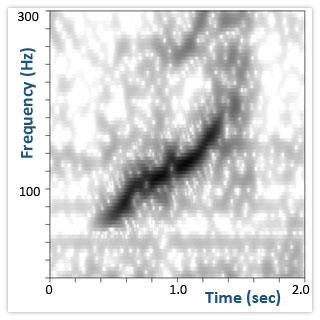
\includegraphics[width= 0.3\textwidth]{images/sound_upcall_quiet.jpg}
\caption{Spectrogram of a rigth whale up-call \cite{CornellWeb} \label{img:upcall}}
\end{figure}
The goal of this work is to present a model capable of detecting the right whale's up-call, which is the most characteristic call of this specie, from the audio detected by the buoys deployed in the sea.
\subsubsection{Datasets and Inputs}\label{datasets-and-inputs}
\begin{comment}
\emph{(approx. 2-3 paragraphs)}

In this section, the dataset(s) and/or input(s) being considered for the
project should be thoroughly described, such as how they relate to the
problem and why they should be used. Information such as how the dataset
or input is (was) obtained, and the characteristics of the dataset or
input, should be included with relevant references and citations as
necessary It should be clear how the dataset(s) or input(s) will be used
in the project and whether their use is appropriate given the context of
the problem.
\end{comment}
The dataset used comes from the competition and consists of 30,000 training samples and 54,503 testing samples. Each candidate is a 2-second .aiff sound clip with a sample rate of 2 kHz. The file "train.csv" gives the labels for the train set. Candidates that contain a right whale call have label=1, otherwise label=0. These clips contain any mixture of right whale calls, non-biological noise, or other whale calls \cite{CornellWeb, CornellWeb2}. 

The training dataset is imbalanced, consisting of approximately 7000 Right Whales samples and 23000 of none Right-Whales samples. We could just balance the samples used or try to use an algorithm that penalizes this imbalance.

The audio is recorded after the buoys auto-detect the characteristic up-call, biasing the dataset to that kind of calls. Thus, it makes sense to detect only that kind of call, which is the most characteristic and most frequently emitted (details on the deployment of the buoys and how the recordings are made in \cite{McDonald2002}). This call (see figure \ref{img:upcall}) has a bandwidth of about 250Hz, fact that will help to reduce information processed to that range of frequencies.



\subsubsection{Solution Statement}\label{solution-statement}


%habia otra de todo tipo de ballenas no?

\begin{comment}
\emph{(approx. 1 paragraph)}

In this section, clearly describe a solution to the problem. The
solution should be applicable to the project domain and appropriate for
the dataset(s) or input(s) given. Additionally, describe the solution
thoroughly such that it is clear that the solution is quantifiable (the
solution can be expressed in mathematical or logical terms) , measurable
(the solution can be measured by some metric and clearly observed), and
replicable (the solution can be reproduced and occurs more than once).
\end{comment}
In order to perform the prediction I will try to implement well-known and widely-implemented models of ConvNets.

One can be the LeNet-5, used for handwritten and machine-printed character recognition. Figure \ref{img:lenet5} shows the structure of the network, composed of 2 convolutional layers, 2 fully connected layers and 2 subsampling or pooling layers.
% which is composed of several layers following the sequence: INPUT -> CONV -> RELU -> SUBS -> CONV -> RELU -> SUBS -> FC -> RELU -> FC, for INPUT, CONV, RELU, SUBS, FC meaning respectively the Input, Convolutional, RELU, Subsampling (or max pooling) and Fully Connected layer.
%\pagebreak
\begin{figure}[htpb!]
\centering
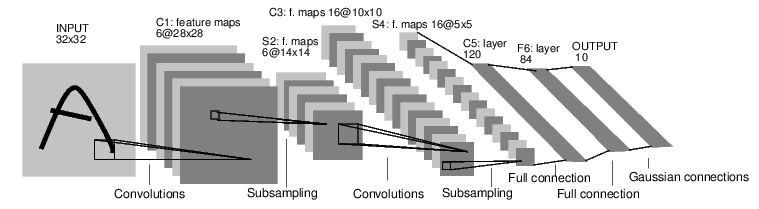
\includegraphics[width= 0.95\textwidth]{images/lenet5}
\caption{LeNet-5 structure \cite{Lecun98} \label{img:lenet5}}
\end{figure}

Other more complex option is the one by Krizhevsky \cite{Krizhevsky12}. Figure \ref{img:imagenet12} shows the structure of the network, composed of 5 convolutional layers, 3 fully connected layers and 3 subsampling or pooling layers.
%, which is composed of several layers following the sequence: INPUT -> CONV -> RELU -> SUBS -> CONV -> RELU -> SUBS -> CONV -> RELU -> CONV -> RELU -> SUBS -> FC -> RELU -> FC, for INPUT, CONV, RELU, SUBS, FC meaning respectively the Input, Convolutional, RELU, Subsampling (or max pooling) and Fully Connected layer.

\begin{figure}[htpb!]
\centering
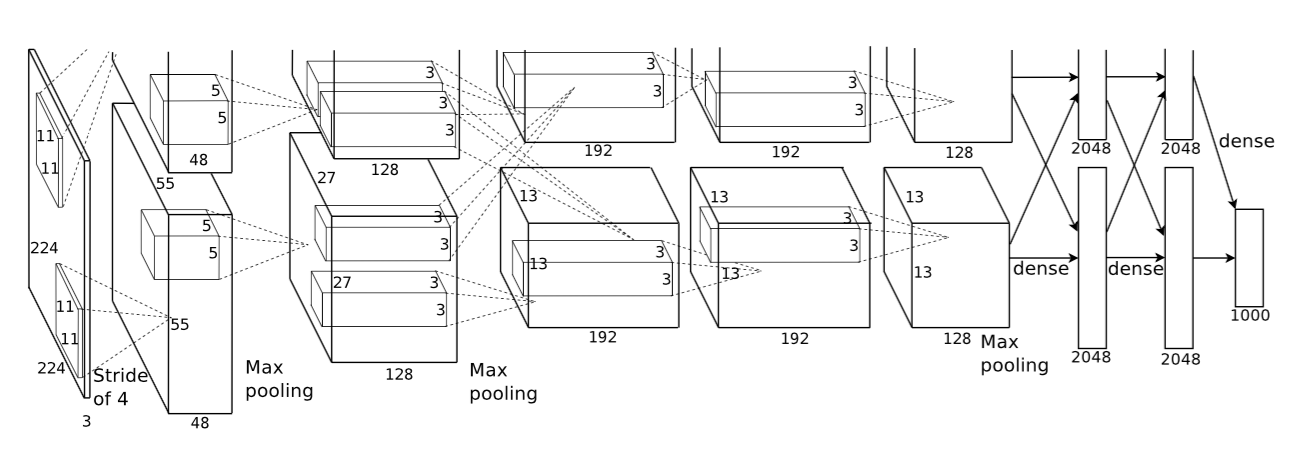
\includegraphics[width= 0.95\textwidth]{images/imagenet12}
\caption{Network structure by Krizhevsky \cite{Krizhevsky12} \label{img:imagenet12}}
\end{figure}


\subsubsection{Benchmark Model}\label{benchmark-model}

\begin{comment}
\emph{(approximately 1-2 paragraphs)}

In this section, provide the details for a benchmark model or result
that relates to the domain, problem statement, and intended solution.
Ideally, the benchmark model or result contextualizes existing methods
or known information in the domain and problem given, which could then
be objectively compared to the solution. Describe how the benchmark
model or result is measurable (can be measured by some metric and
clearly observed) with thorough detail.
\end{comment}
I will try to compare the performance of the most popular ConvNets (i.e. LeNet-5 proposed by Lecun \cite{Lecun98} or the winner of the 2010 and 2012 \imagenet \, proposed by Krizhevsky \cite{Krizhevsky12}) with the performance of the winning model of the competition which is based on Gradient Boosting (SluiceBox: \href{https://github.com/nmkridler/moby}{Github}) and the Daniel Nouri's model based on Krizhevsky's 2012 ILSVRC ConvNet model \cite{Krizhevsky12} (\href{https://speakerdeck.com/dnouri/practical-deep-neural-nets-for-detecting-marine-mammals/}{source}), which first inspired this work.

The Area Under the Curve (AUC) (see the Evaluation metrics section\ref{evaluation-metrics}) of these models in the public leaderboard was:
\begin{itemize}
	\item SluiceBox: 0.98410 (1st position)
	\item Nouri: 0.98061 (6th position with 1/4 times the submission of the winner)
\end{itemize}

Nevertheless, I will not be able compare the performance of my models to these results. The reason is that I do not have the test labels and also, the public leaderboard data test used is slightly different for each participant. I will try two different approaches:
\begin{enumerate}
	\item assuming that there are enough complete data samples (train dataset), trying to increase the accuracy as much as possible (this will be the main option)
	\item assuming the predictions generated by the winning model as test labels and them as reference to compare our model with
\end{enumerate}
\begin{comment}

However, as the competition is closed, I cannot access the test labels and compare the performance to others algorithms. Two options sound plausible:
\begin{itemize}
	\item divide the train dataset into: train, cross-validation and test dataset
	\item use the winning algorithm to generate an estimation of the test labels and so increase the amount of data for training.
\end{itemize}
\end{comment} 
%pero no podemos comparar directamente porque no tenemos el test dataset

\subsubsection{Evaluation Metrics}\label{evaluation-metrics}
\begin{comment}
\emph{(approx. 1-2 paragraphs)}

In this section, propose at least one evaluation metric that can be used
to quantify the performance of both the benchmark model and the solution
model. The evaluation metric(s) you propose should be appropriate given
the context of the data, the problem statement, and the intended
solution. Describe how the evaluation metric(s) are derived and provide
an example of their mathematical representations (if applicable).
Complex evaluation metrics should be clearly defined and quantifiable
(can be expressed in mathematical or logical terms).
\end{comment}

The main evaluation metric for this project will be that used in the Kaggle competition, this is the \textbf{Area Under the Curve (AUC)}, where the Curve is the ROC curve.

The \textbf{receiver operating characteristic (ROC)} curve is a graphical plot that illustrates the performance of a binary classifier system as its discrimination threshold is varied. The curve is created by plotting the true positive rate (TPR) against the false positive rate (FPR) at various threshold settings.

The true-positive rate is also known as sensitivity, recall or probability of detection. The false-positive rate is also known as the fall-out or probability of false alarm. 

The ROC curve is thus, the sensitivity as a function of fall-out. In general, if the probability distributions for both detection and false alarm are known, the ROC curve can be generated by plotting the cumulative distribution function (area under the probability distribution from $-\infty$  to the discrimination threshold) of the detection probability in the y-axis versus the cumulative distribution function of the false-alarm probability in x-axis (see figure \ref{img:ROC})\cite{wikiROC}

\begin{figure}[htpb!]
\centering
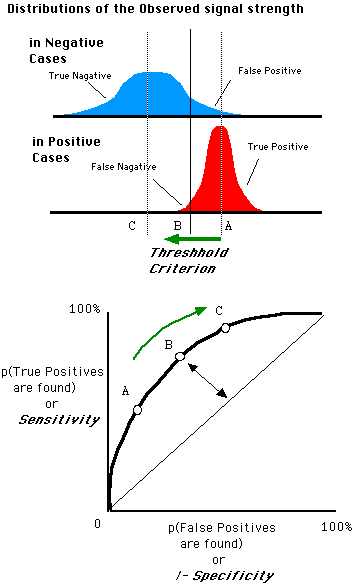
\includegraphics[width= 0.4\textwidth]{images/ROCfig}
\caption{ROC curve graphic explanation \cite{wikiwand} \label{img:ROC}}
\end{figure}

Another important measure can be the \textbf{error rate} vs iterations for a different batch sizes. The error rate used can be the percentage of wrong classified samples.

It can be also interesting to use the \textbf{confusion matrix}, which is a more detailed version of the ROC curve. The confusion matrix is a table that shows the predicted labels for each of the true input labels.



\subsubsection{Project Design}\label{project-design}
\begin{comment}
\emph{(approx. 1 page)}

In this final section, summarize a theoretical workflow for approaching a solution given the problem. Provide thorough discussion for what strategies you may consider employing, what analysis of the data might
be required before being used, or which algorithms will be considered
for your implementation. The workflow and discussion that you provide
should align with the qualities of the previous sections. Additionally,
you are encouraged to include small visualizations, pseudocode, or
diagrams to aid in describing the project design, but it is not
required. The discussion should clearly outline your intended workflow
of the capstone project.
\end{comment}


\begin{enumerate}
	\item sound samples exploration
	\item spectrogram generation and image processing (contrast, appropriate dimensions...)
	\item separation of dataset into training, cross-validation and test dataset and save into pickle 
	\item select ConvNets model and adjust parameters
	\begin{itemize}
		\item define structure of the ConvNet adequate for my images: depth of layers, and stride and patch size of filters and pooling layers
		\item AUC vs epochs (or training iterations), Error vs epochs, for different batch sizes
		\item tune the model using regularization and decaying learning rate		
	\end{itemize}
	\item compare the performance of winning model using the reduced version train and test dataset extracted form the train dataset
\end{enumerate}

%\begin{center}\rule{3in}{0.4pt}\end{center}
\begin{comment}

\textbf{Before submitting your proposal, ask yourself. . .}

\begin{itemize}
\itemsep1pt\parskip0pt\parsep0pt
\item
  Does the proposal you have written follow a well-organized structure
  similar to that of the project template?
\item
  Is each section (particularly \textbf{Solution Statement} and
  \textbf{Project Design}) written in a clear, concise and specific
  fashion? Are there any ambiguous terms or phrases that need
  clarification?
\item
  Would the intended audience of your project be able to understand your
  proposal?
\item
  Have you properly proofread your proposal to assure there are minimal
  grammatical and spelling mistakes?
\item
  Are all the resources used for this project correctly cited and
  referenced?
\end{itemize}
\end{comment}






\bibliography{../../../../../media/mabelvj/Darsena/DropboxUbuntu/Dropbox/PhD/library}

\end{document}
